\documentclass{ercisbeamer}

\title{Spacing}
\subtitle{Effective Studying}
\author{Sven Ligensa}
\institute{European Research Center for Information Systems (ERCIS)}
\date{\today}

\begin{document}

\setbgimage{00_resources/jungle_brain}
\begin{frame}
    \begin{tbox}
        \titlepage
    \end{tbox}
\end{frame}
\setbgimage{}

\begin{frame}{Contents}
    \tableofcontents
\end{frame}


\setbgimage{08_resources/Spacing_50}
\section{Overview}
\begin{frame}{Overview}
    \begin{tbox}
        \begin{itemize}
            \item \red{Letting time pass between study sessions}
            \item Leads to forgetting ($\rightarrow$ Forgetting Curve) = Desirable difficulty
            \item Anything you want to remember must be periodically recalled from memory
            \item Crucial aspect of everyday experiences
            \item Combine with Retrieval
            \item Reach back to retrieve prior material \\ $\rightarrow$ See how knowledge relates to what you learned later
        \end{itemize}
        \vspace{3.5em} \hspace{0.1em}\\
    \end{tbox}
        \begin{picture}(0,0)
            \put(310,15){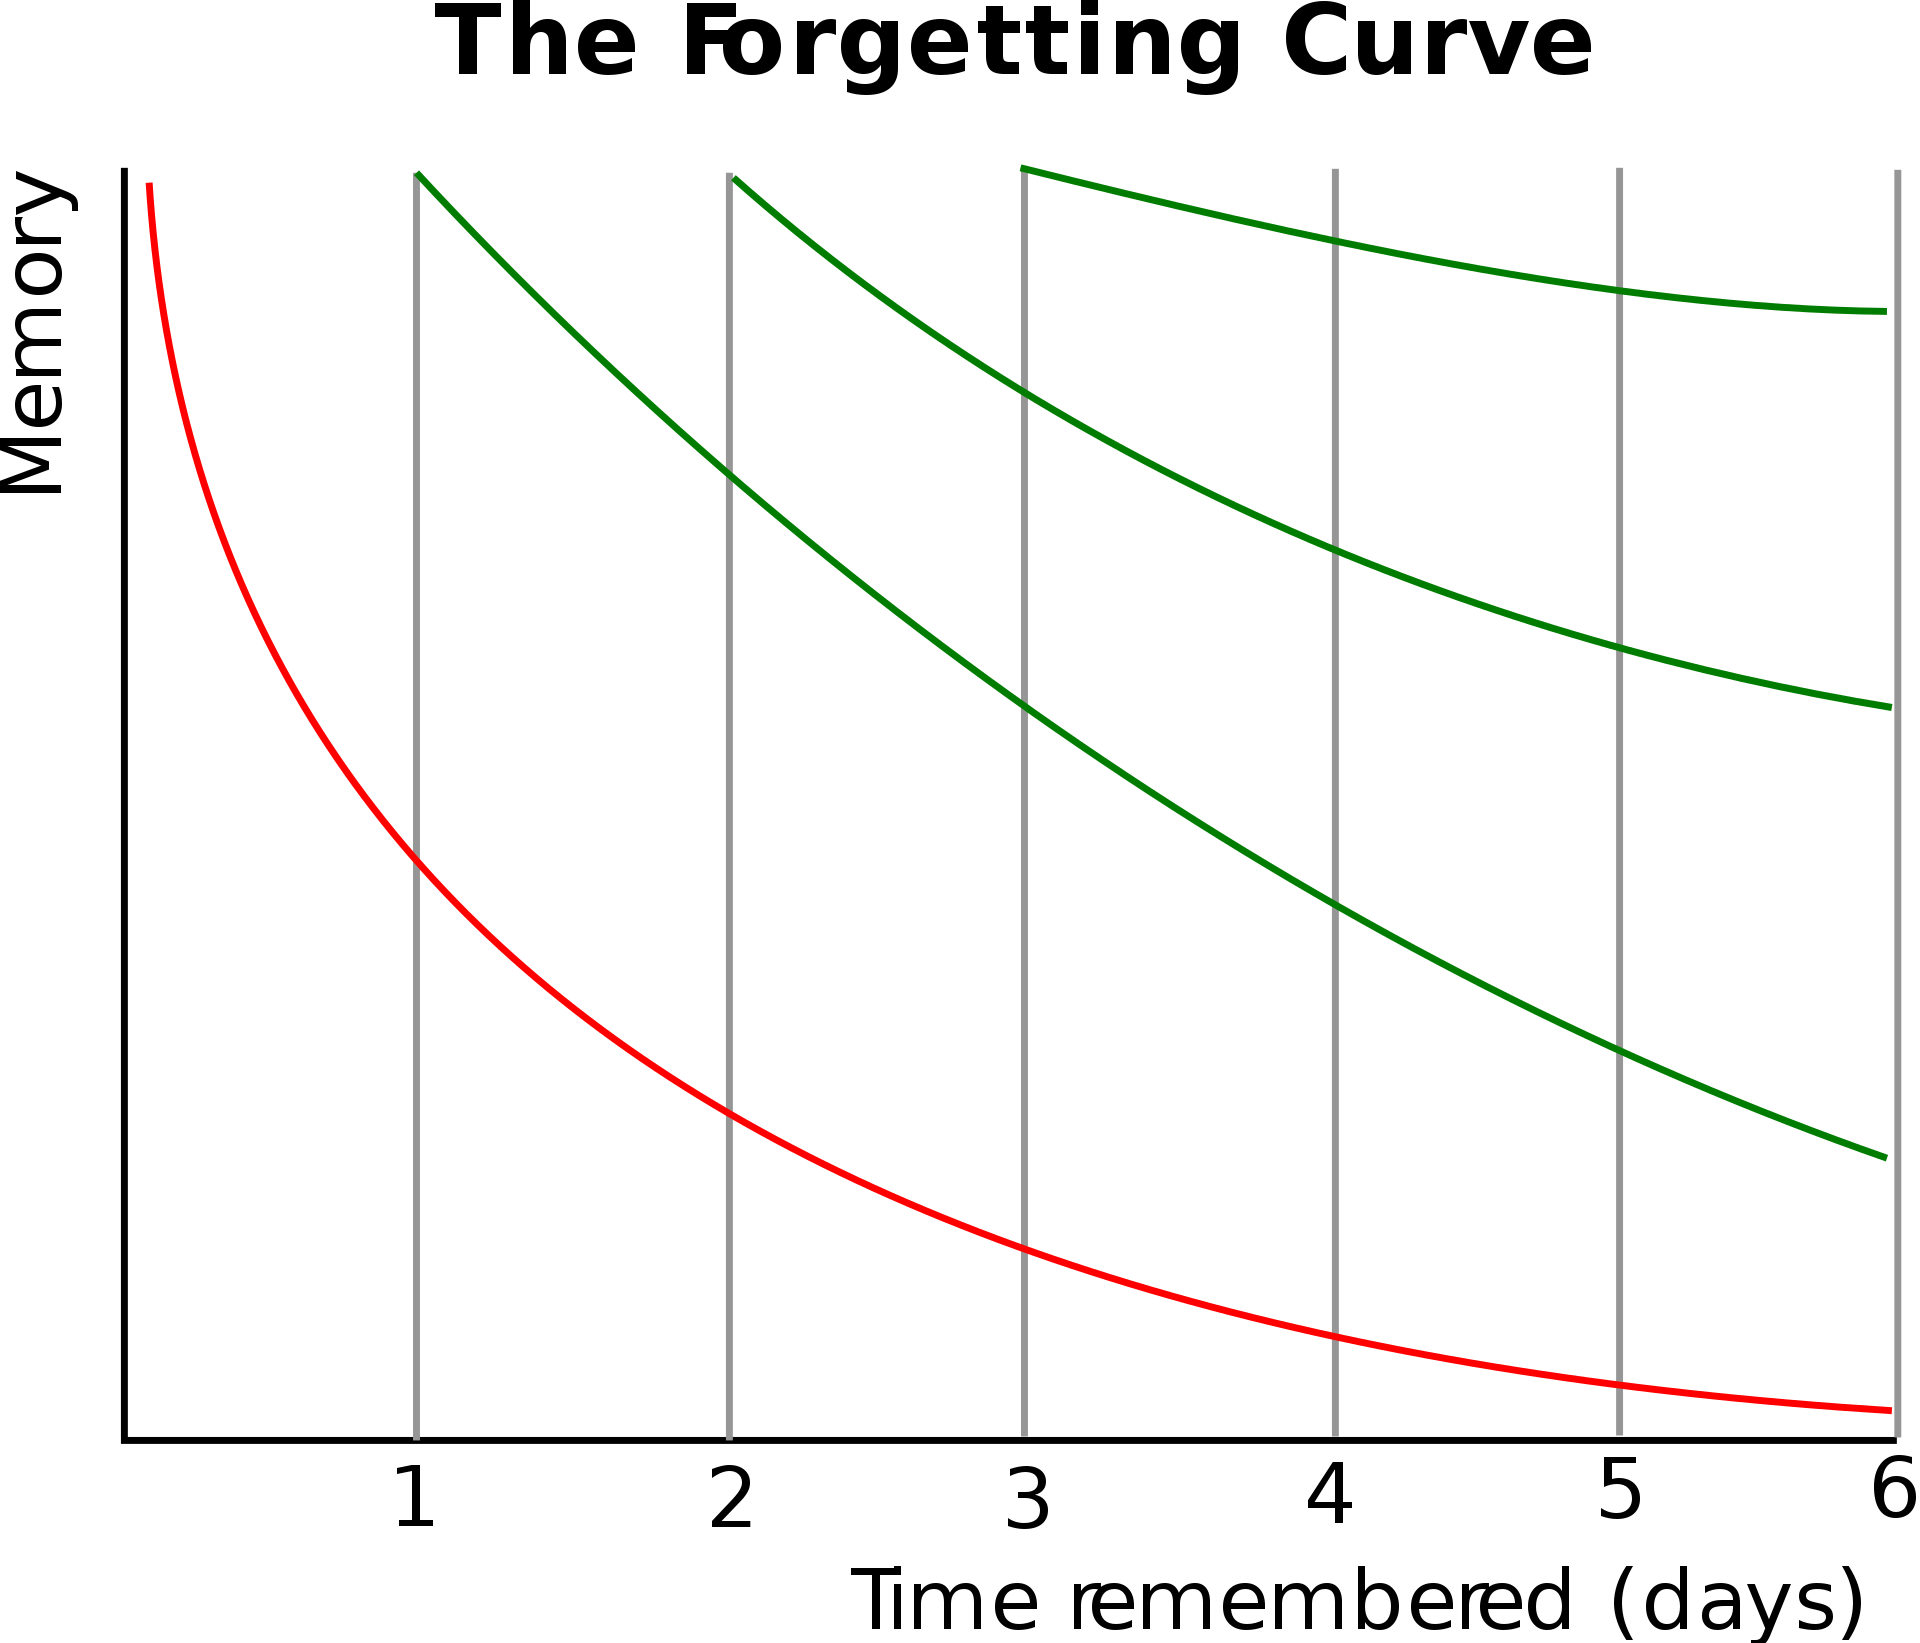
\includegraphics[width=0.25\paperwidth]{08_resources/forgetting_curve.png}}
        \end{picture}
\end{frame}

\section{Length of Interval}
\begin{frame}{Length of Interval}
    \begin{tbox}
        \begin{itemize}
            \item Enough that practice does not become mindless repetition
            \begin{itemize}
                \item Little forgetting should have set in
                \item Not so much that retrieval essentially involves relearning the material
            \end{itemize}
            \item Mastery of material $\uparrow$ $\Rightarrow$ Length of interval $\uparrow$
            \begin{itemize}
                \item Do not drop important information completely
            \end{itemize}
            \item Depends on study material
        \end{itemize}
    \end{tbox}
    
    \hspace{2em}
    
    \begin{tbox}
        \begin{itemize}
            \item \citet{karpicke11}
            \begin{itemize}
                \item \emph{``Repeated \red{spaced retrieval} had \red{powerful effects} on retention, but the \red{relative schedule} of repeated tests had \red{no discernible impact}.''}
                \item \emph{``It is well known that \red{increasing} the \red{absolute spacing} between repetitions \red{improves retention}, especially in the long term.''}
            \end{itemize}
        \end{itemize}
    \end{tbox}
\end{frame}
\setbgimage{}

\section{Advantages}
\begin{frame}{Advantages}
    \begin{itemize}
        \item Learning has time to \positive{consolidate} into cohesive representation in the brain for long-term memory
        \item \positive{Interrupts forgetting}
    \end{itemize}
\end{frame}


\section{Implementation}
\begin{frame}{Implementation}
    \begin{itemize}
        \item Set aside some time every week \red{throughout the semester} to study
        \item Physical Flashcards: Manually (e.g. via Leitner system)
        \item Digital Flashcards: Implemented \red{algorithm} (can often be tuned for personal preference)
        \item Questions + Answers: \red{Revision calendar}
    \end{itemize}
\end{frame}


\section{Now You!}
\begin{frame}{Now You!}
    \begin{itemize}
        \item \emph{How exactly do you want to implement Spacing into your study routine? \\ Consider what works best with your Retrieval strategy.}
        \item \emph{When do you want to start studying for the next examination phase?}
        \item \emph{Apply spacing by reviewing this material in the next days.}
    \end{itemize}
\end{frame}


\section*{Outlook}
\begin{frame}{Outlook}
    \begin{enumerate}
        \item \positive{Introduction}
        \vspace{.5em}
        \item \positive{Illusions of Knowing}
        \item \positive{Understanding the Brain}
        \item \positive{Learning}
        \item \positive{Desirable Difficulties}
        \item \positive{Effective vs. Ineffective Learning Strategies}
        \vspace{.5em}
        \item \positive{Retrieval}
        \item \positive{Spacing}
        \item Next: \red{Variation and Interleaving}
        \item \grey{Mental Models}
        \item \grey{Memory Cues}
    \end{enumerate}
\end{frame}

\thankyou{Happy Learning!}{sven.ligensa@uni-muenster.de}

\sources

\end{document}
